\section{Лекция номер 8}
\subsection{Еще (не)много равномерной сходимости}

\textbf{Признак Дини.} 
Пусть у нас есть:
\begin{itemize}
    \item $K$ -- компакт
    \item $u_n \in C(K)$ и $u(n) \geqslant 0$ -- непрерывные неотрицательные функции на нем
    \item $S(x) := \sum\limits_{n = 1}^\infty u_n(x) \in C(K)$ -- сумма ряда тоже непрервная функция
\end{itemize}
Тогда ряд сходится равномерно.
\begin{proof}
    Введем $S_n = \sum\limits_{k = 1}^n u_k(x)$ -- частичная сумма, $r_n(x) = S(x) - S_n(x) = \sum\limits_{k = n+1}^\infty u_k(x)$ -- все остальное.
    Знаем, что $r_n(x) \in C(K)$ как разность непрерывных, и $r_n(x)$ монотонно убывают, так как $S_n(x)$ монотонно возрастают.
    Надо доказать, что $r_n \rightrightarrows 0$, то есть \[ \forall \varepsilon > 0  \;\; \exists n \;\; \forall m \geqslant n \quad |r_m(x)| < \varepsilon \;\; \forall x \in K \]
    Заметим, что модуль нам не нужен, так как $r_n(x) > 0$, а также достаточно расмматривать только $n$-тый член ряда, ведь $r_n(x)$ убывают:
    \[ \forall \varepsilon > 0  \;\; \exists n \quad r_n(x) < \varepsilon \;\; \forall x \in K \]
    Предположим противное и зафиксируем тот $\varepsilon$, для которого все портится.
    Тогда $\forall n \; \exists x_n \in K : r_n(x_n) \geqslant \varepsilon$. 
    Так как $x_n \in K$, мы можем выбрать подпоследовательность, сходящуюся к точке из компакта: $x_{n_k} \to x_0 \in K$.
    Тогда $\forall m \;\; r_m(x_{n_k}) \to r_m(x_0)$. 
    При фиксированном $m$ мы можем найти такое достаточно большое $n_k$, что $r_m(x_{n_k}) \geqslant r_{n_k}(x_{n_k})$, ведь $r_n(x)$ убывают.
    Мы знаем, что $r_{n_k}(x_{n_k}) \geqslant \varepsilon$, поэтому $r_m(x_{n_k}) \geqslant \varepsilon$ и по предельному переходу $r_m(x_0) \geqslant \varepsilon$.
    Это уже что-то непонятное, так как тогда в точке $x_0$ остаток не стремится к 0, и $S_n(x_0) \nrightarrow S(x_0)$. Противоречие. 
\end{proof}

 Теперь обсудим свойства равномерно сходящихся последовательностей и рядов.
 Эти свойства покажут нам, что условие равномерной сходимости очень полезное, и именно благодаря нему мы можем менять местами два предела, пределел с интегрированием и предел с дифференцированием.

\vspace*{5mm}

 \begin{theorem}
     Пусть $f_n, f : E \to \R$, $a$ -- предельная точка $E$, $f_n \rightrightarrows f$ на $E$ и $\lim\limits_{x \to a} f_n(x) =: b_n \in \R$. 
     Тогда $\lim b_n, \lim\limits_{x \to a} f(x)$ существуют, конечны и равны.
     В частности $\lim\limits_{x \to a} \lim\limits_{n \to \infty} f_n(x) =  \lim\limits_{n \to \infty} \lim\limits_{x \to a} f_n(x)$.
 \end{theorem}
 \begin{proof}
     Согласно критерию Коши: \[ \forall \varepsilon > 0 \;\; \exists N \;\; \forall n, m \geqslant N \;\; \forall x \in E \quad |f_n(x) - f_m(x)| < \varepsilon \]
     \quad Устремим $x$ к $a$ и получим, что: \[ \forall \varepsilon > 0 \;\; \exists N \;\; \forall n, m \geqslant N \quad |b_n - b_m| < \varepsilon  \]
     \quad Это критерий Коши для последовательности $b_n$, следовательно, у нее есть предел, обозначим его за $b \in \R$.
     Докажем, что $\lim\limits_{x \to a} f(x) = b$. Оценим их разность c помощью неравенства треугольника:
     \[ |f(x) - b| \leqslant |f_n(x) - f(x)| + |b_n - f_n(x)| + |b - b_n| \]
     \quad Заметим, что первое и третье слагаемые будут $< \varepsilon$ при достаточно больших $n$, а второе будет $< \varepsilon$ в некоторой окрестности $a$.
     А именно: \begin{itemize}
         \item Первое слагаемое будет $< \varepsilon$ при $n \geqslant N_1$ из определения равномерной сходимости. 
         \item Второе слагаемое будет $< \varepsilon$ при $|x - a| < \delta$, так как $f_n(x) \to b_n$ и $\delta$ взята как раз из этого предела.
         \item Третье слагаемое будет $< \varepsilon$ при $n \geqslant N_2$, так как $b_n \to b$.
     \end{itemize} 
     \quad Таким образом, $|f(x) - b| < 3\varepsilon$ при $|x - a| < \delta$. Это и означает, что $\lim\limits_{x \to a} f(x) = b$.
 \end{proof}

\vspace*{7mm}

Можно определить аналогичную вещь для рядов.

 \begin{theorem}
     Пусть $u_n: E \to \R, a$ -- предельная точка, $\sum\limits_{n=1}^\infty u_n(x)$ равномерно сходится и $\lim\limits_{x \to a} u_n(x) = c_n$.
     Тогда $\lim\limits_{x \to a} \sum\limits_{n=1}^\infty u_n(x) = \sum\limits_{n=1}^\infty c_n = \sum\limits_{n=1}^\infty \lim\limits_{x \to a} u_n(x)$ и этот ряд сходится.
     То есть мы можем менять местами предел с суммой.
 \end{theorem}
 \begin{proof}
    Чтобы воспользоваться предыдущей теоремой, введем 
    \begin{gather*}
        f_n(x) := \sum\limits_{k=1}^n u_k(x) \rightrightarrows f(x) := \sum_{n=1}^\infty u_n(x) \\
        b_n: = \lim_{x \to a} f_n(x) = \lim_{x \to a} \sum_{k=1}^n u_k(x)
    \end{gather*}
    \quad Заметим, что так как сумма $\sum\limits_{k=1}^n u_k(x)$ конечная, мы можем менять местами сумму с пределом:
    \[ b_n: = \lim_{x \to a} \sum_{k=1}^n u_k(x) = \sum_{k=1}^n \lim_{x \to a} u_k(x) = \sum_{k=1}^n c_k  \]
    
    \quad Тогда согласно теореме существует $\lim\limits_{n \to \infty} b_n$, то есть ряд $\sum\limits_{n = 1}^\infty c_n$ сходится, и $\lim\limits_{n \to \infty} b_n = \lim\limits_{x \to a} f(x)$, то есть $\sum\limits_{n = 1}^\infty c_n = \lim\limits_{x \to a} \sum\limits_{n = 1}^\infty u_n(x)$.
 \end{proof}
 \begin{follow}
     Если $u_n$ непрерывны в точке $a$ и $\sum\limits_{n = 1}^\infty u_n(x)$ равномерно сходится, то $\sum\limits_{n = 1}^\infty u_n(x)$ непрерывна в точке $a$.
 \end{follow}
\begin{proof}
    Непрерывность $u_n$ в точке $a$, говорит нам о том, что $c_n = \lim\limits_{x \to a} u_n(x) = u_n(a)$.

    \quad Тогда \[ \lim\limits_{x \to a} \sum\limits_{n=1}^\infty u_n(x) = \sum\limits_{n=1}^\infty c_n = \sum\limits_{n=1}^\infty u_n(a)   \]
    \quad Это и есть непрерывность $\sum\limits_{n = 1}^\infty u_n(x)$ в точке $a$.
\end{proof}

\begin{notice}
    Равномерная непрерывность тут важна. 

    Пример: $f_n(x) = x^n : [0, 1] \to \R$ -- непрерывные функции. Но предельная функция \[ f(x) = \begin{cases}
        0, & \text{при $x \in [0, 1)$} \\
        1, & \text{при $x = 1$}
    \end{cases} \]
    не будет непрерывной.
 \end{notice}

\vspace*{10mm}

Теперь разберемся с интегрированием.

\begin{theorem}
    Пусть $f_n \in C[a, b]$, $f_n \rightrightarrows f$ на $[a, b]$ и $c \in [a, b]$. 
    Тогда $\int_c^x f_n(t)dt \rightrightarrows \int_c^x f(t)dt$.

    В частности $\lim\limits_{n \to \infty} \int_c^x f_n(t)dt = \int_c^x \lim\limits_{n \to \infty} f_n(t)dt$.
\end{theorem}

\begin{proof}
    Введем $F_n(x) := \int_c^x f_n(t)dt$ и $F(x) := \int_c^x f(t)dt $. 
    
    \quad Будем оценивать разность:
    \begin{gather*}
        \begin{split}
            |F_n(x) - F(x)| &= \left|\int_c^x f_n(t)dt - \int_c^x f(t)dt \right| \\
            &\leqslant \int_c^x |f_n(t) - f(t)|dt \text{ (занесли под один интеграл и внесли модуль) } \\
            &\leqslant (x - c) * \max_{t \in [c, x]} |f_n(t) - f(t)| \text{ (самая простая оценка интеграла) } \\
            &\leqslant (b - a) * \max_{t \in [c, x]} |f_n(t) - f(t)| \text{ (еще увеличили длину) }\\
            &= (b - a) * \underbrace{\sup_{t \in [c, x]} |f_n(t) - f(t)|}_{\to 0 \text{ т.к. равн. сх-ть}} \text{ (на отрезке $\max = \sup$) }
        \end{split}
    \end{gather*}
    Наша разность оценилась как что-то стремящееся к 0 и не зависящее от $x$. Это и есть равномерная сходимость.
\end{proof}

\vspace*{7mm}

Можно определить аналогичную вещь для рядов.

\begin{follow}
    Если $u_n \in C[a, b]$ и $\sum\limits_{n=1}^\infty u_n(x)$ равномерно сходится, то $\int_c^x \sum\limits_{n=1}^\infty u_n(t) dt = \sum\limits_{n=1}^\infty \int_c^x u_n(t) dt$.
\end{follow}
\begin{proof}
    В предыдущей теореме $f_n(t) = \sum\limits_{n=1}^\infty u_n(t)$.
\end{proof}

\begin{notice}
    Поточечной сходимости не хватает.
    
    \quad Пример: $f_n(x) = nxe^{-nx^2}$ на $[0, 1]$.

    \quad Очевидно, что $\forall x \;\; f_n(x) \to 0$ при $n \to \infty$. Но \[ \int_0^1 f_n(x)dx = \frac{-e^{-nx^2}}{2}\Big|_0^1 = \frac{1 - e^{-n}}{2} \nrightarrow 0 = \int_0^1 f(x)dx \]
\end{notice}

\vspace*{10mm}

Ну и наконец дифференцирование.

\begin{theorem} Пусть у нас есть:
     \begin{itemize}
        \item $f_n \in C^1[a, b]$
        \item $f_n$ сходятся в какой-то точке $c \in [a, b]$, то есть $f_n(c) \to A$
        \item $f_n' \rightrightarrows g$ на $[a, b]$
    \end{itemize}
    Тогда $f_n \rightrightarrows f$ на $[a, b]$, где $f \in C^1[a, b]$ и $f' = g$. В частности, $\lim\limits_{n \to \infty} f_n'(x) = (\lim\limits_{n \to \infty} f_n(x))'$.
\end{theorem}
\begin{proof}
    Посмотрим на следующие интегралы:
    \begin{gather*}
        \int_c^x g(t)dt = \int_c^x \lim\limits_{n \to \infty} f_n'(t)dt \underbrace{=}_{\text{пред. теор.}} \lim\limits_{n \to \infty} \int_c^x  f_n'(t)dt = \\
        = \lim\limits_{n \to \infty} (f_n(x) - f_n(c)) \underbrace{=}_{\text{исп. кон-ть $\lim f_n(c)$}} \lim\limits_{n \to \infty} f_n(x) - \lim\limits_{n \to \infty} f_n(c) = f(x) - A \\ 
        \\
        \Rightarrow f(x) = A + \int_c^x g(t)dt \Rightarrow f \in C^1[a, b] \text{ и } f'(x) = g(x)
    \end{gather*}
    \quad Вообще говоря, последний переход -- это теорема Барроу, так как согласно ней интеграл от непрерывной функции это функция дифференцируемая.

    \quad Осталось проверить равномерную сходимость $f_n(x)$ к $f(x)$.
    Заметим, что у нас есть следующие тождества:
    \begin{gather*}
        f_n(x) = \int_c^x f'_n(t)dt + f_n(c) \\
        f(x) = \int_c^x g(t)dt + A
    \end{gather*}
    По предыдущей теореме $\int_c^x f'_n(t)dt \rightrightarrows \int_c^x g(t)dt$. 
    По условию $f_n(c) \to A$, это не зависит от $x$, поэтому $f_n(c) \rightrightarrows A$.
    Таким образом, $f_n(x) \rightrightarrows f(x)$.
\end{proof}

\vspace*{7mm}

Можно определить аналогичную вещь для рядов.

\begin{follow}
    Пусть у нас есть: \begin{itemize}
        \item $u_n \in C^1[a, b]$
        \item $\sum\limits_{n=1}^\infty u_n$ сходится в какой-то точке $c \in [a, b]$, то есть $\sum\limits_{n=1}^\infty u_n(c) \to A$
        \item $\sum\limits_{n=1}^\infty u_n'(x)$ равномерно сходится на $[a, b]$
    \end{itemize}
    Тогда $\sum\limits_{n=1}^\infty u_n(x)$ равномерно сходится к дифференцируемой функции и $\left(\sum\limits_{n=1}^\infty u_n(x)\right)' = \sum\limits_{n=1}^\infty u_n'(x)$. 
\end{follow}
\begin{proof}
    Чтобы воспользоваться теоремой, введем $f_n(x) := \sum\limits_{k=1}^n u_k(x)$. 
    Конечная сумма дифференцируемых функций это тоже дифференцируемая функция, поэтому $\sum\limits_{k=1}^n u_k(x) \in C^1[a, b]$. 
    Производная конечной суммы это сумма производных, поэтому $f_n'(x) = \sum\limits_{k=1}^n u_k'(x)$, что по условию $\rightrightarrows \sum\limits_{k=1}^\infty u_k'(x) =: g(x)$.

    \quad Применив предыдущую теорему, получаем, что $f_n \rightrightarrows f$, где $f' = g$. Это означает, что ряд равномерно сходится и $\left(\sum\limits_{n=1}^\infty u_n(x)\right)' = g(x) = \sum\limits_{n=1}^\infty u_n'(x)$.
\end{proof}

\begin{notice}
    Тут важна именно равномерная сходимость производных, равномерной сходимости изначальных функций недостаточно.

    \quad Пример: $\sum\limits_{n=1}^\infty \frac{\sin nx}{n^2}$ равномерно сх-ся по признаку Вейерштрасса, так как $|\frac{\sin nx}{n^2}| \leqslant \frac{1}{n^2}$.
    Но ряд из производных $\sum\limits_{n=1}^\infty (\frac{\sin nx}{n^2})' = \sum\limits_{n=1}^\infty \frac{\cos nx}{n}$ расходится при $x = 0$. 
    То есть мы получили, что почленное дифференцирование приводит к расходящемуся ряду, что не может быть производной сходящегося ряда.
\end{notice}

\subsection{Степенные ряды}
\begin{conj}
    Степенным рядом называется ряд вида $\sum\limits_{n=0}^\infty a_n(z - z_0)^n$, где $a_n, z, z_0 \in \C$.
\end{conj}
\begin{notice}
    Сделав замену $w := z - z_0$, получаем ряд $\sum\limits_{n=0}^\infty a_n w^n$, в котором $z_0 = 0$. 
    Зачастую именно такая форма более удобна, а к общей форме можно легко перейти сдвигом.
\end{notice}

\vspace*{5mm}

\begin{theorem} (Абеля)
    Если $\sum\limits_{n=0}^\infty a_n z^n$ сходится при $z_0 \neq 0$, то он абсолютно сходится при $|z| < |z_0|$.    
\end{theorem}
\begin{proof}
    Если ряд $\sum\limits_{n=0}^\infty a_n z_0^n$ сходится, у нас должно выполняться необходимое условие сходимости: $a_nz_0^n \to 0$.
    Значит, $a_nz_0^n$ ограничены: $|a_nz_0^n| \leqslant M$. 
    Тогда при $|z| < |z_0|$ наш ряд ограничен геометрической прогрессией: $|a_nz^n| = |a_nz_0^n| * |\frac{z}{z_0}|^n \leqslant M|\frac{z}{z_0}|^n$.
    Она является сходящейся, поэтому наш ряд сходится по признаку сравнению.
\end{proof}

Таким образом, данная теорема утверждает, что если ряд сходится в какой-то точке $z_0$, то отметив ее на комплексной плоскости, мы получим, что во всех точках, лежащих внутри круга с радиусом равным $|z_0|$, ряд будет сходиться.

Отметим одно очевидное следствие.

\begin{follow}
    Если $\sum\limits_{n=0}^\infty a_n z^n$ расходится при $z_0 \neq 0$, то он расходится и при $|z| > |z_0|$.
\end{follow}
\begin{proof}
    От противного: если бы он сходился при $z$, то по предыдущей теореме сходился бы и при $z_0$.
\end{proof}

\vspace*{5mm}

Все это наталкивает нас на мысль, что существует такой круг, что внутри него ряд сходится, а вне -- расходится.
Определим это формально.

\begin{conj}
    Радиус сходимости степенного ряда $\sum\limits_{n=0}^\infty a_n z^n$ -- это такое число $R \in [0, +\infty]$, что $\forall z : |z| < R$ ряд сходится, а $\forall z : |z| > R$ ряд расходится.
\end{conj}

\begin{conj}
    Круг сходимости степенного ряда $\sum\limits_{n=0}^\infty a_n (z - z_0)^n$ -- открытый круг радиуса $R$ (радиус сходимости) в точке $z_0$.
\end{conj}

\begin{center}
    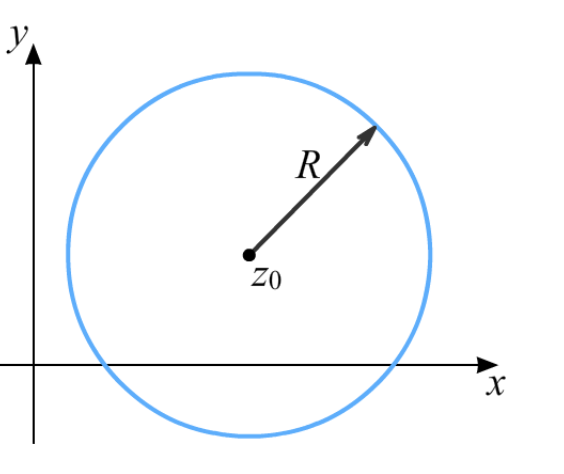
\includegraphics[scale=0.4]{circle.png}    
\end{center}

\begin{notice}
    Во всех точках круга сходимости ряд сходится. 
    Вне замыкания круга сходимости ряд расходится.
    Про границу мы ничего утверждать не можем. 
\end{notice}

\vspace*{10mm}

Давайте поймем, что любой степенной ряд имеет радиус сходимости.

\begin{theorem} (Формула Коши-Адамара)
    Всякий степенной ряд имеет радиус сходимости, причем его можно посчитать по формуле $R = \frac{1}{\overline{\lim\limits_{n \to \infty}} \sqrt[n]{|a_n|}}$.
\end{theorem}
\begin{proof}
    Применим к ряду $\sum\limits_{n = 0}^\infty a_n z^n$ признак Коши, а именно посчитаем $q^* = \overline{\lim\limits_{n \to \infty}} \sqrt[n]{|a_nz^n|}$. 
    (Вообще в признаке Коши под корнем нет модуля, но добавить его это законно, так как если сходится абсолютно, то сходится и обычно, а если абсолютно расходится, то по признаку Коши нет необходимого условия сходимости, то есть и обычно расходится.)

    Распишем $q^*:$ \[ q^* = \overline{\lim_{n \to \infty}} \sqrt[n]{|a_nz^n|} = \overline{\lim_{n \to \infty}} (\sqrt[n]{|a_n|} * |z|) = |z| * \overline{\lim_{n \to \infty}} \sqrt[n]{|a_n|}   \]
    Тогда согласно признаку Коши: \begin{itemize}
        \item Если $q^* < 1$, то ряд сходится $\Rightarrow$ если $|z| < \frac{1}{\overline{\lim\limits_{n \to \infty}} \sqrt[n]{|a_n|}}$, то ряд сходится.
        \item Если $q^* > 1$, то ряд сходится $\Rightarrow$ если $|z| > \frac{1}{\overline{\lim\limits_{n \to \infty}} \sqrt[n]{|a_n|}}$, то ряд сходится.
    \end{itemize}
    Это и говорит нам о том, что $R = \frac{1}{\overline{\lim\limits_{n \to \infty}} \sqrt[n]{|a_n|}}$ -- радиус сходимости.
\end{proof}

\begin{notice}
    Мы попутно поняли, что внутри круга сходимости ряд абсолютно сходится.
\end{notice}

\vspace*{7mm}
Поприменяем данную формулу на простых примерах.

\begin{examples}
    \begin{enumerate}
        \item $\sum\limits_{n=0}^\infty n!z^n$. 
        По формуле $R = \frac{1}{\overline{\lim\limits_{n \to \infty}} \sqrt[n]{n!}}$. 
        Так как предел этой последовательности существует, мы можем убрать знак верхнего предела: $R = \frac{1}{\lim\limits_{n \to \infty} \sqrt[n]{n!}} \thicksim \frac{1}{\lim\limits_{n \to \infty} (\frac{n}{e}\sqrt[2n]{2\pi n})} = \frac{1}{+\infty} = 0$.
        
        $\Rightarrow$ ряд сходится только в 0.
        \item $\sum\limits_{n=0}^\infty \frac{z^n}{n!}$. 
        По формуле $R = \frac{1}{\overline{\lim\limits_{n \to \infty}} \sqrt[n]{1/n!}}$.
        Опять же можем убрать верхний предел: $R = \frac{1}{\lim\limits_{n \to \infty} \sqrt[n]{1/n!}} = \lim\limits_{n \to \infty} \sqrt[n]{n!} = +\infty$.

        $\Rightarrow$ ряд сходится при всех $z \in \C$.
        \item $\sum\limits_{n=0}^\infty \frac{z^n}{n^p}$, где $p \in \R$.
        По формуле (сразу заменяем на обычный предел): $R = \frac{1}{\lim\limits_{n \to \infty} \sqrt[n]{1/n^p}} = \lim\limits_{n \to \infty} \sqrt[n]{n^p} = 1$.
        
        $\Rightarrow$ ряд сходится при $|z| < 1$ и расходится при $|z| > 1$.

        Этот пример также демонстрирует тот факт, что на границе круга ряд может как сходиться, так и расходиться: \begin{itemize}
            \item Если $p = 2$, то $|\frac{z}{n^2}| \leqslant \frac{1}{n^2}$ при $|z| \leqslant 1 \Rightarrow$ ряд сходится при $|z| \leqslant 1$.
            \item Если $p = 1$ и $z = 1$, то ряд расходится, так как является гармоническим.
            \item Если $p = 1$ и $z = -1$, то ряд сходится, так как является рядом Лейбница.
            \item Если $p = 0$, то при $|z| = 1$ ряд расходится, так как $|z| \nrightarrow 0$.
        \end{itemize}
    \end{enumerate}    
\end{examples}

\vspace*{10mm}
Оказывается, что внутри круга еще есть равномерная сходимость.

\begin{theorem}
    Пусть $R$ -- радиус сходимости ряда $\sum\limits_{n=0}^\infty a_nz^n$ и $0 < r < R$. 
    Тогда в круге $|z| \leqslant r$ ряд сходится равномерно.
\end{theorem}
\begin{proof}
    $r < R \Rightarrow \sum\limits_{n=0}^\infty a_nr^n$ сходится абсолютно (этот факт был в одном из замечаний).
    Если $|z| \leqslant r$, то $|a_nz^n| \leqslant |a_nr^n|$. 
    Тогда по признаку Вейерштрасса ряды $\sum\limits_{n=0}^\infty a_nz^n$ и $\sum\limits_{n=0}^\infty |a_nz^n|$ сходятся равномерно.
\end{proof}
\begin{follow}
    Сумма степенного ряда непрерывна в круге сходимости.
\end{follow}
\begin{proof}
    Пусть мы хотим доказать непрерывность в точке $z_0$, принадлежащей кругу сходимости.
    Возьмем $r: 0 < |z_0| < r < R$, тогда ряд равномерно сходится в круге $|z| \leqslant r \Rightarrow$ его сумма непрерывна в точках $|z| < r \Rightarrow$ в точке $z_0$ есть непрерывность.
\end{proof}

\begin{theorem} (Абеля) \;
    Пусть $R$ -- радиус сходимости и ряд сходится при $z = R$. 
    Тогда ряд сходится равномерно на $[0, R]$.
\end{theorem}
\begin{proof}
    Рассмотрим ряд $\sum\limits_{n = 0}^\infty a_n x^n$, где $x \in [0, R]$.
    Мы можем его переписать как $\sum\limits_{n = 0}^\infty a_n x^n = \sum\limits_{n = 0}^\infty a_n R^n (\frac{x}{R})^n$. 
    Заметим, что $\sum\limits_{n = 0}^\infty a_n R^n$ сходится (по условию), причем равномерно, так как от $x$ не зависит. 
    Также последовательность $(\frac{x}{R})^n$ равномерно ограничена (например, числом 1) и монотонна как геометрическая прогрессия. 
    Тогда по признаку Абеля ряд $\sum\limits_{n = 0}^\infty a_n x^n$ сходится равномерно на $[0, R]$.
\end{proof}

\begin{follow}
    Пусть $R$ -- радиус сходимости и ряд сходится при $z = R$. 
    Тогда его сумма непрерывна на $[0, R]$ и $\lim\limits_{x \to R-} \sum\limits_{n=0}^\infty a_nx^n = \sum\limits_{n=0}^\infty a_nR^n$.
\end{follow}
\begin{proof}
    По предыдущему следствию знаем, что сумма будет непрерывна. 
    Тогда равенство $\lim\limits_{x \to R-} \sum\limits_{n=0}^\infty a_nx^n = \sum\limits_{n=0}^\infty a_nR^n$ и есть условие непрерывности, так как справа стоит значение в точке $R$.
\end{proof}

\vspace*{10mm}

Докажем простую техническую лемму.

\begin{lemma}
    Пусть $x_n, y_n \in \R$ и $\lim x_n \in (0, +\infty)$. 
    Тогда $\overline{\lim} \, x_ny_n = \lim x_n * \overline{\lim} \, y_n$.
\end{lemma}
\begin{proof}
    Введем $A := \lim x_n, B := \overline{\lim} \, y_n, C := \overline{\lim} \, x_ny_n$.

    \quad Выберем подпоследовательность $y_{n_k} \to B$. 
    Тогда $x_{n_k} \to A$ по свойству предела $x_n$.
    Итого, $x_{n_k}y_{n_k} \to AB$. 
    Это какой-то частичный предел последовательности $x_ny_n$, он очевидно не превосходит наибольшего $\Rightarrow AB \leqslant C$.

    \quad Теперь выберем подпоследовательность $x_{n_k}y_{n_k} \to C$. 
    Тогда $x_{n_k} \to A$ по свойству предела $x_n$.
    Итого, $y_{n_k} \to \frac{C}{A}$.
    Это какой-то частичный предел последовательности $y_n$, он очевидно не превосходит наибольшего $\Rightarrow \frac{C}{A} \leqslant B \Rightarrow C \leqslant AB$.

    \quad Таким образом, $AB = C$.
\end{proof}

\begin{follow}
    Радиусы сходимости рядов $\sum\limits_{n=0}^\infty a_n z^n, \sum\limits_{n=0}^\infty a_n \frac{z^{n+1}}{n+1}$ и $\sum\limits_{n=0}^\infty n a_n z^{n-1}$ равны.
\end{follow}
\begin{proof}
    Будем рассматривать ряды $\sum\limits_{n=0}^\infty a_n z^n, \sum\limits_{n=0}^\infty a_n \frac{z^n}{n+1}$ и $\sum\limits_{n=0}^\infty n a_n z^{n}$. 
    Второй и третий ряд мы домножили на константу, понятно, что радиус сходимости от этого не изменился.
    Для этих рядов уже все очевидно (пользуемся нашей леммой): \[ R_1 = \frac{1}{\overline{\lim} \sqrt[n]{|a_n|}} \quad R_2 = \frac{1}{\overline{\lim} \sqrt[n]{\frac{|a_n|}{n+1}}} = R_1 \quad R_3 = \frac{1}{\overline{\lim} \sqrt[n]{n|a_n|}} = R_1   \]
\end{proof}

\vspace*{5mm}

Также внутри круга сходимости мы можем почленно интегрировать.

\begin{theorem}
    Пусть $R$ -- радиус сходимости ряда $f(x) = \sum\limits_{n = 0}^\infty a_n(x - x_0)^n$.
    
    Тогда при $|x - x_0| < R \quad \int_{x_0}^x f(t)dt = \sum\limits_{n = 0}^\infty a_n \frac{(x - x_0)^{n+1}}{n+1}$ и этот ряд имеет тот же радиус сходимости.
\end{theorem}
\begin{proof}
    На $[x_0, x]$ ряд для $f$ сходится равномерно, так как этот отрезок полностью попал в круг сходимости $\Rightarrow$ можем интегрировать почленно:
    \begin{gather*}
        \int_{x_0}^x f(t)dt = \int_{x_0}^x \sum_{n=0}^\infty a_n(t - x_0)^n dt = \sum_{n=0}^\infty \int_{x_0}^x a_n(t - x_0)^n dt =  \\
        = \sum_{n = 0}^\infty a_n \frac{(t - x_0)^{n+1}}{n+1}\Big|_{x_0}^x = \sum_{n=0}^\infty a_n \frac{(x - x_0)^{n+1}}{n+1} 
    \end{gather*}
    Этот ряд имеем тот же радиус сходимости по предыдущему следствию.
\end{proof}